\section{Subsystem Decomposition}
The \texttt{DriveIT System} can be split into five main sub systems - the \texttt{WindowsClient}, \texttt{CarQuery}, \texttt{Web}, \texttt{WebAPI} and \texttt{EntityFramework} sub systems. 
These subsystems are described below. 

\subsection{The DriveIT System}
\begin{figure}[H]
	\centering
	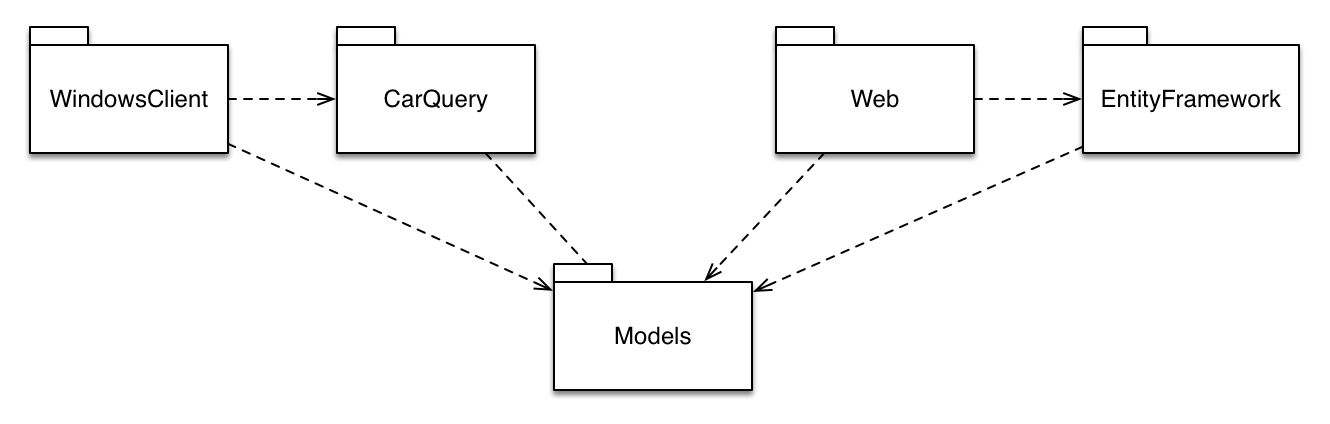
\includegraphics[width=\textwidth]{Figures/DriveITSubsystemDecomposition}\\
	\caption{Subsystems of the \texttt{DriveIT System}.}
\end{figure}

\subsection{Persistence subsystem (EntityFramework)} 
This sub system manages storing and retrieving Entity objects using the Entity Framework and its serialisation functionality.\\
The serialised Entities are stored in a Microsoft SQL database which is hosted on Microsoft Azure. The sub system provides the \texttt{DriveIT Web API} (mentioned below) deserialised Entities, which uses these to provide the backend for other sub systems using the API.\\
The subsystem supports retrieving all Entities of a given type, a specific Entity using its unique ID and retrieving an Entity on its relation to other Entities. 
\begin{figure}[H]
	\centering
	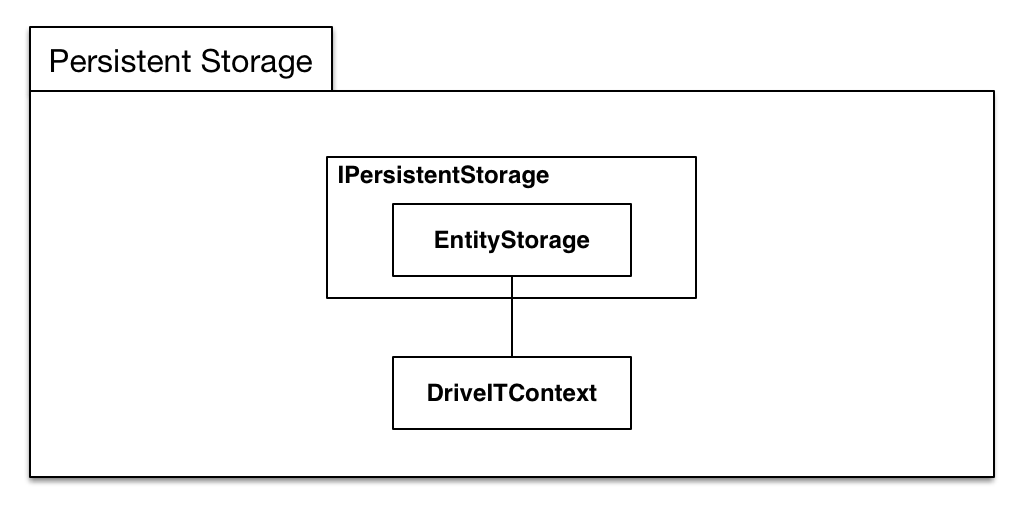
\includegraphics[width=\textwidth]{Figures/EntityFrameworkSubsystemDecomposition}
	\caption{Subsystems of the EntityFramework Subsystem.}
\end{figure}

\subsection{Web API} 
\todo{maybe more should as this are still some kind of analysis.}
The \texttt{DriveIT Web API} provides public communication with the persistence subsystem and also handles authorisation of users of the sub system.\\
The subsystem, which is built on ASP.NET Web API, provides access to the persistence sub system using specific URL routes and enforces authorisation so unauthorized users, and users with different user roles, only have limited access to the data of the \texttt{DriveIT System}.\\ 
Every table in the persistence module must therefore be supported by the Web API, although not every table is available to every user.\\
The \texttt{DriveIT Web API} is comprised of a series of modules for serialising the Model Entities into \texttt{JSON}\footnote{\url{http://en.wikipedia.org/wiki/JSON}} or \texttt{XML}\footnote{\url{http://en.wikipedia.org/wiki/XML}} and transferring these via a \texttt{REST} interface accessible using \texttt{HTTP}. \\
These modules are built into the ASP.NET Web API framework, and are not handled in our code.\\

The Web API consists of several controllers which uses a static class to translate \texttt{DTO's}\footnote{\url{http://en.wikipedia.org/wiki/Data_transfer_object}} into entities and vice versa. It is also the controllers that checks for special cases, e.g. when a customer wants to update or delete a comment, and it is not allowed to change other peoples comments.


\subsection{Windows Client} 
\begin{figure}[H]
	\centering
	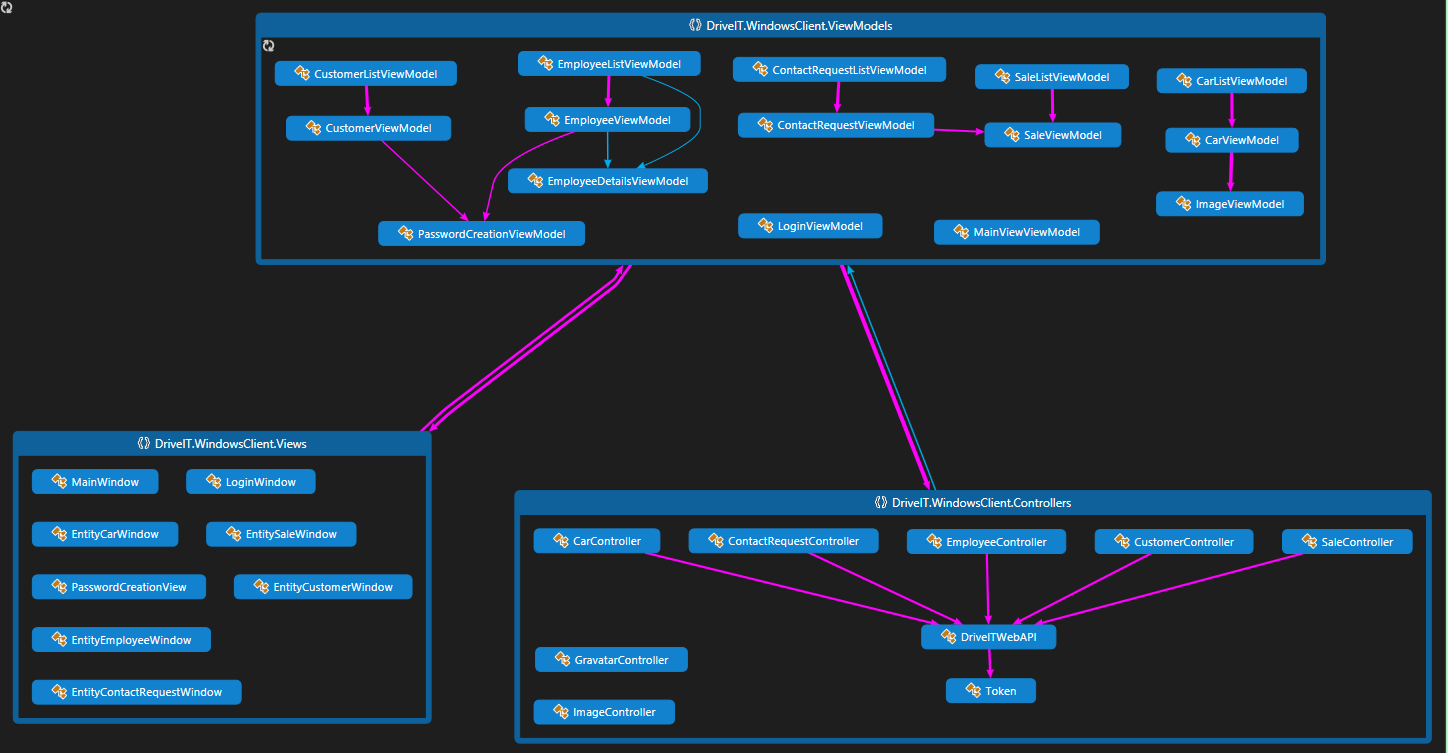
\includegraphics[width=\textwidth]{Figures/WindowsClientCodeMap}
	\caption{The Code Map of the Windows Client}
	\label{fig:WindowsClientCodeMap}
\end{figure}
The Windows Client is used by the employees, to manipulate data in the system. Depending on their role Employee or Administrator They can Create, Read, Update and Delete all entities except for creating \texttt{ContactRequest}, which only can be created through the \texttt{DriveIT Web Client}.\\
The employee logs into the client with his or hers username and password, and can then via an user interface manipulate data in the system.\\
The subsystem is made out of three main systems: The DriveIT.Views, the DriveIT.ViewModels and the DriveIT.Controllers.\\
The DriveIT.Views contains the user interface written in with Microsofts WPF framework. The DriveIT.ViewModels contains the ViewModels which holds data which is bound to the Views following Microsoft's \emph{Model View ViewModel} architectural pattern. Viewmodels for entities are often created in the form EntityListViewModel and EntityViewModel, but a few extra viewmodels exists for extra views such as the LoginViewModel and the PasswordCreationViewModel.\\
The DriveIT.Controllers section contains the controllers which transforms data and sends and receives HTTP Requests to/from the \texttt{DriveIT Web API}. Images are uploaded to \emph{Azures Blob Storage} and therefore does not contact the API. Another controller to notice is the \texttt{GravatarController} which takes email strings and converts it to a link to that emails Gravatar profile url.

\subsection{Web Client}
The \texttt{DriveIT Web Client} is accessable through the internet, whereas it is being used by non-registered users and customers, who already have registered themselves through the web client and logged on. The web client is being used to search for cars, that are being sold by the company using the \texttt{DriveIT System}, CRUD comments (if the customer is logged in, else it's only read), CRD contact requests, read orders and read employees (contact tab). A customer is also able to create, read and update information regarding their own user account.
The web client is based on the ASP.NET MVC framework, that is implementing the MVC design pattern. The subsystem is made of three components: Models, Views and Controllers. The views contains the user interface and is written in cshtml, which is a mix of C$\sharp$ and HTML code. The models contains lists of database records and the controllers are responsible for giving the models, filled with database records, to the views, for them to display the data in the model.

\subsection{CarQuery} 
This subsystem is a collection of classes that enable the rest of the \texttt{DriveIT System} to fill out missing information about cars from the CarQuery API.\\
The sub system is used by an employee when creating a new car. The subsystem mainly consists of a \texttt{JSON} deserialiser that communicates with the \texttt{CarQuery REST API} and another class that receives a Car object and fills out the missing attributes using the deserialised JSON data. \\
The employee fills out the information he/she knows about the car and the system then narrows its information search against the \texttt{CarQuery REST API}.
\begin{figure}[H]
	\centering
	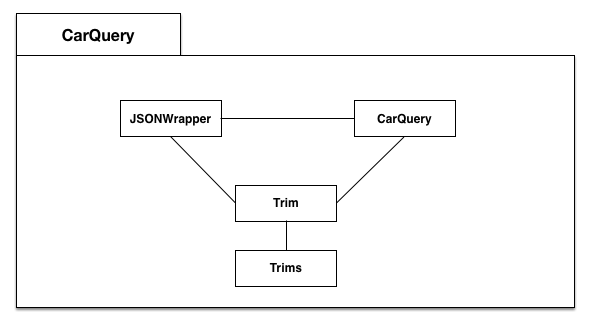
\includegraphics[width=\textwidth]{Figures/CarQuerySubsystemDecomposition}\\
	\caption{Subsystems of the CarQuery Subsystem.}
\end{figure}